\section{Results}

\begin{figure}
    \centering
    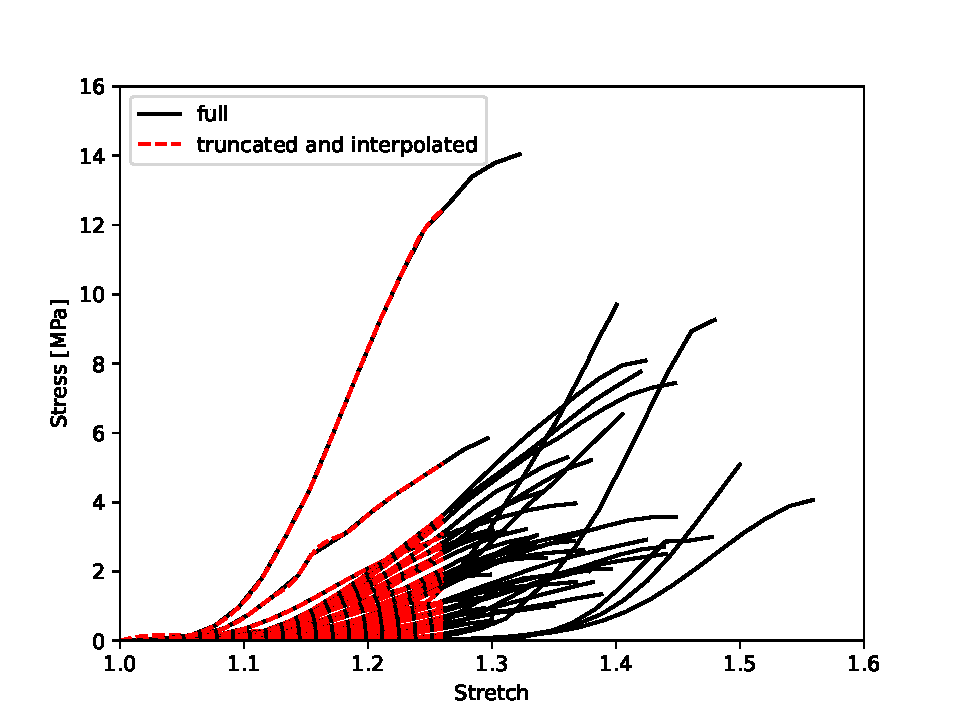
\includegraphics[width=\linewidth]{skinstression/images/truncated-and-interpolated-curves.pdf}
    \caption[Truncated and spline interpolated curves]{
        The strain-stress curves (black) were truncated and interpolated (dotted red)
        using non-uniform, interpolating splines on the stretch values of the curve with the lowest maximum stretch.
    }
    \label{fig:trunc_interp_curves}
\end{figure}

\subsection{Participants}

Earlier studies (refs) include 18 individuals (5 men, 4 women, and 6 unknown).
Abdomen data was excluded, because the strain-stress curves differ significantly from the thigh.
All thigh data is included, which is different from the original study, where only the 48 latest samples were used.
These considerations result in data including 15 individuals (5 men, 4 women, 3 unknown).
Ages range from 61 to 94.
Skin tissue is cut from the thigh and cut in multiple pieces of roughly the same shape.\marginpar{protocol?}
From every skin tissue piece, strain-stress curves are measured.
The number of measured strain-stress curves range from 1 to 13.
The source of data is summarized in \cref{fig:source_of_data}.

\begin{figure*}
    \centering
    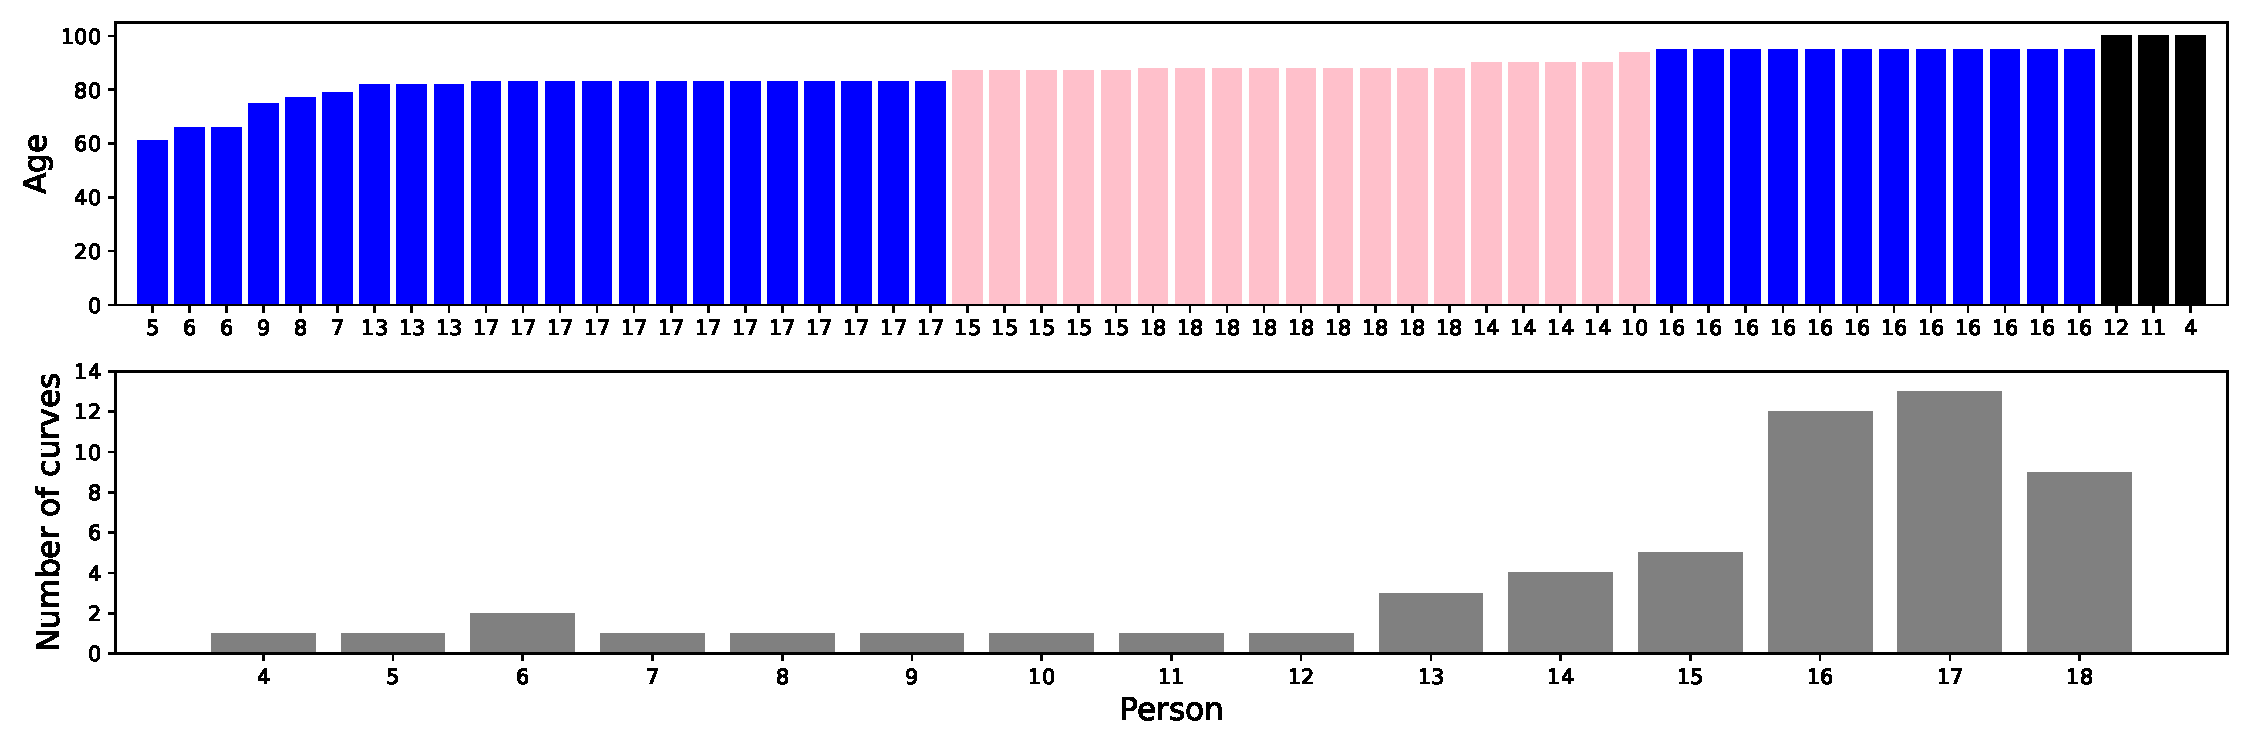
\includegraphics[width=\linewidth]{skinstression/images/age_distribution.pdf}
    \caption[Source of data]{
        The selected individuals and their sex, age and number of strain-stress curves.
        Top panel: shows the age and sex distribution. Blue, pink and black denote male, female and unknown sex.
        In fact, the age of person 12, 11, and 4 are unknown.
        Bottom panel: shows the number of curves per person.
    }
    \label{fig:source_of_data}
\end{figure*}

\subsection{Predictor pre-selection}
\subsubsection{Exponential}
An exponential fit to \cref{eq:exp} is shown in \cref{fig:exp_fits}.
$R^2 = \num{0.9497}$.
The exponent is not able to fit the plateau that is often exhibited near maximum stretch.

\begin{figure}
    \centering
    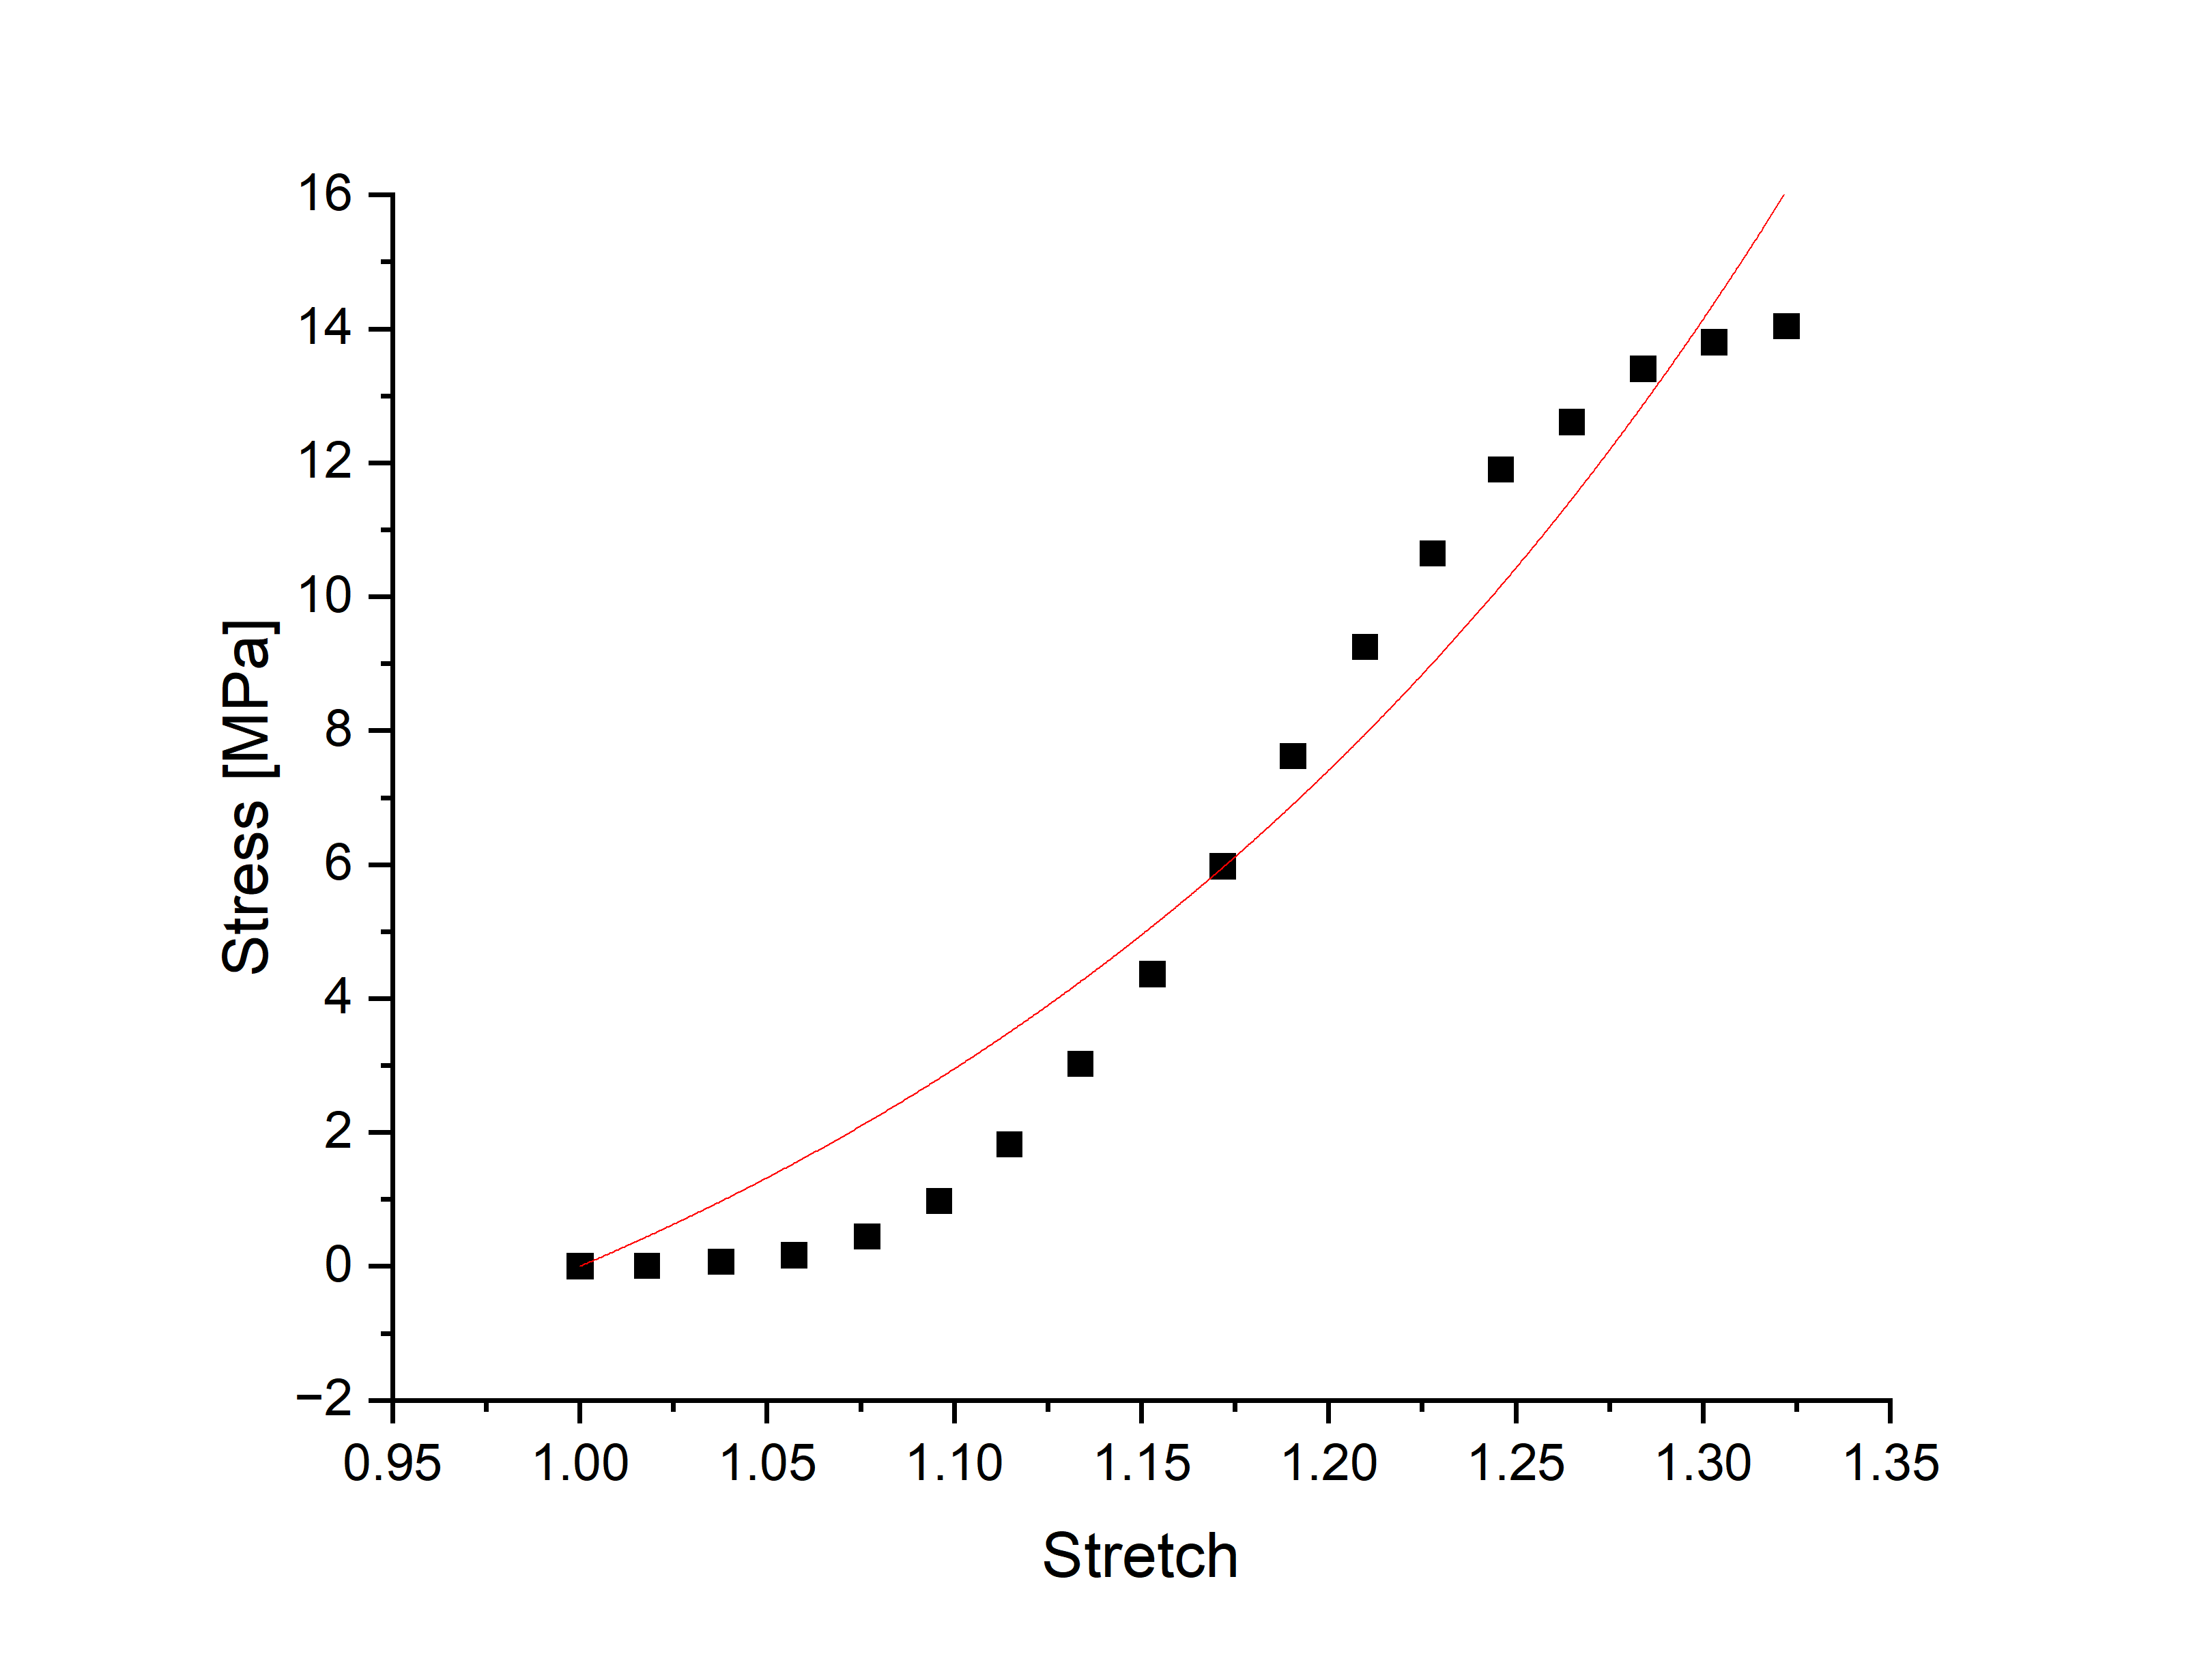
\includegraphics[width=0.5\linewidth]{skinstression/images/exp-fits/exponential.png}
    \caption[Exponential fit]{
        Exponential fit with \cref{eq:exp} (red) for one stress-strain curve (black).
        Fit parameters were $G_0=\qty{23.8\pm4.0}{\mega\pascal\per\stretch}$, and $\lambda=\qty{4.1\pm 1.0}{\stretch}$.
        $R^2=\num{0.9497}$.
    }
    \label{fig:exp_fits}
\end{figure}

\subsubsection{PCA}
The PCA fit for every truncated and interpolated strain-stress curve is depicted in \cref{fig:pca_fits}.
For every fit, $R^2$ is calculated with respect to the interpolated and truncated data.
On average, $\overline{R^2} \approx \num{0.9927 \pm 0.0022}$.
Due to the nature of PCA, the exponential part of the curves that rise later is not included in the making of the fit.

\begin{figure*}
    \centering
    \foreach \c in {1,2,...,61}{%
            \IfFileExists{skinstression/images/pca-fits/sample_\c.pdf} {%
                \includegraphics[width=0.24\linewidth]{skinstression/images/pca-fits/sample_\c.pdf}
            }{%
                % files do not exist, so nothing to do
            }
        }
    \caption[PCA fits]{
        PCA fits for every truncated and interpolated strain-stress curve.
        The interpolated measurements (blue) are estimated by the PCA curve (red) along with their $R^2$.
        PCA is done on all available thigh data.
        Note that the vertical axes are not equal.
    }
    \label{fig:pca_fits}
\end{figure*}

\subsubsection{Logistic curve}
The logistic curve fit for every strain-stress curve is shown in \cref{fig:logistic_fits}.
For every fit, $R^2$ is calculated.
On average, $\overline{R^2} \approx \num{0.9979 \pm 0.0039}$.

\begin{figure*}
    \centering
    \foreach \c in {1,2,...,61}{%
            \IfFileExists{skinstression/images/logistic-fits/sample_\c.pdf} {%
                \includegraphics[width=0.24\linewidth]{skinstression/images/logistic-fits/sample_\c.pdf}
            }{%
                % files do not exist, so nothing to do
            }
        }
    \caption[Logistic fits]{
        Logistic fits (red) and their $R^2$ for every strain-stress curve (black).
        Note that the vertical axes are not equal.
    }
    \label{fig:logistic_fits}
\end{figure*}

Because the logistic curve describes the stress-strain data more accurate than PCA or the exponential, it will be used from now on.

\subsubsection{Label density smoothing}
The labels were smoothed using LDS using gaussian kernels.
All kernels had a size of 30 and a standard deviation of 3.
The distribution bins were manually set to $(\sigma_{\mathrm{max},\mathrm{min}}, \sigma_{\mathrm{max},\mathrm{max}}, s_{\sigma_\mathrm{max}}) = (0, 15, 0.01) \unit{\mega\pascal}$,
$(E_{\mathrm{max},\mathrm{min}}, E_{\mathrm{max},\mathrm{max}}, s_{E_\mathrm{max}}) = (0, 50, 0.1) \unit{\mega\pascal\per\stretch}$, and
$(\gamma_{c,\mathrm{min}}, \gamma_{\mathrm{max},\mathrm{max}}, s_{\gamma_\mathrm{max}}) = (1, 1.5, 0.001) \unit{\stretch}$,
where $s$ is the bin width.
The smoothed distribution is shown in \cref{fig:skin_lds}.

\begin{figure*}
    \centering
    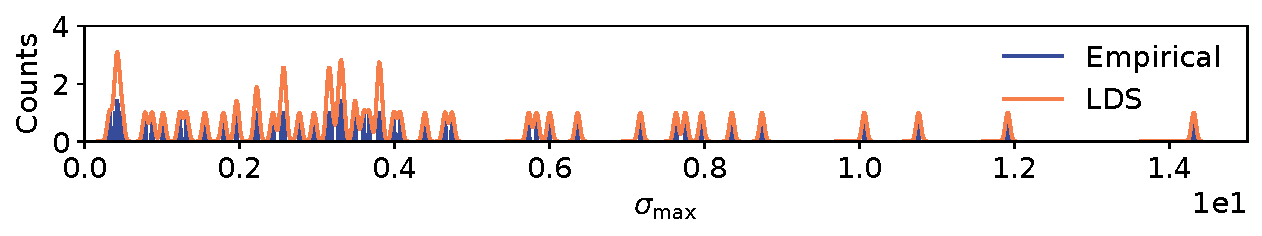
\includegraphics{skinstression/images/lds/a.pdf} \\
    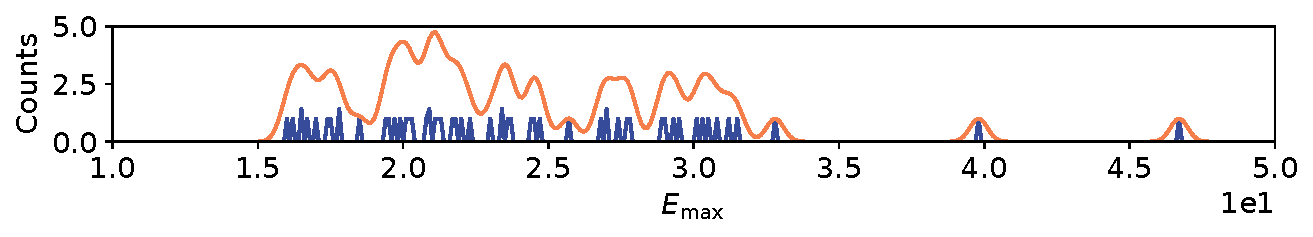
\includegraphics{skinstression/images/lds/k.pdf} \\
    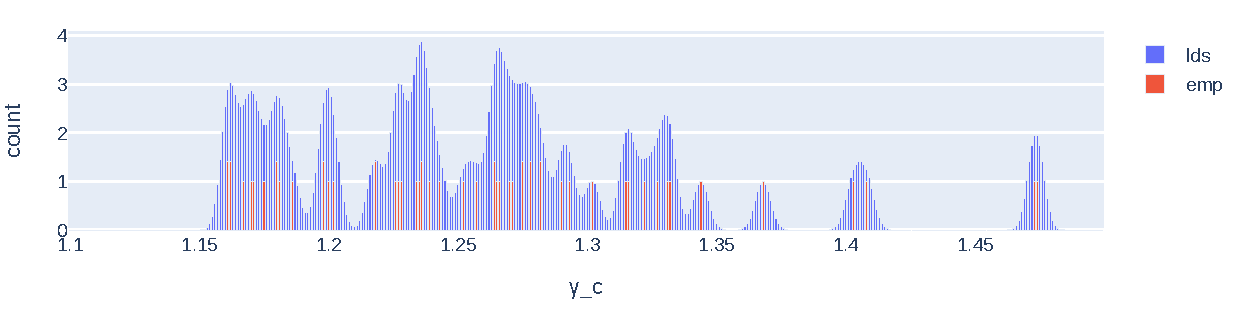
\includegraphics{skinstression/images/lds/xc.pdf}
    \caption[Original target and LDS distrutions]{
        Empirical target distribution (red) and LDS distribution (blue) for $\sigma_\mathrm{max}$, $E_\mathrm{max}$, and $\gamma_c$.
        LDS aims to fill the gaps between the actual measurements.
        LDS also extrapolates target distributions.
        For all targets, the kernel size was 30 units, and the standard deviation 3 units.
        The bin width were \num{0.01}, \num{0.1}, and \num{0.001} units for $\sigma_\mathrm{max}$, $E_\mathrm{max}$, and $\gamma_c$, respectively.
    }
    \label{fig:skin_lds}
\end{figure*}

%%%%%%%%%%%%%%%%%%%%%%%%%%%%
% IMAGE QUALITY
%%%%%%%%%%%%%%%%%%%%%%%%%%%%

\subsection{Image quality}
Presumably, the model will yield erroneous predictions if images of bad quality are provided.
Moreover, the measurement was not always done in the same order, \ie from the lowest to the highest tissue or vice versa.
Therefore, two image quality measurements were explored: Shannon entropy and kurtosis.

The kurtosis of some image stacks were used to validate the image quality by eye, see \cref{fig:skin_kurtosis_depth}.
The entropy of the same image stacks as for kurtosis were used to validate the image quality by eye, see \cref{fig:skin_entropy_depth}.

For reasons explained in \cref{sec:disc_ent_vs_kur}, entropy is further used to choose the top quality images from every stack.

\begin{figure*}
    \centering
    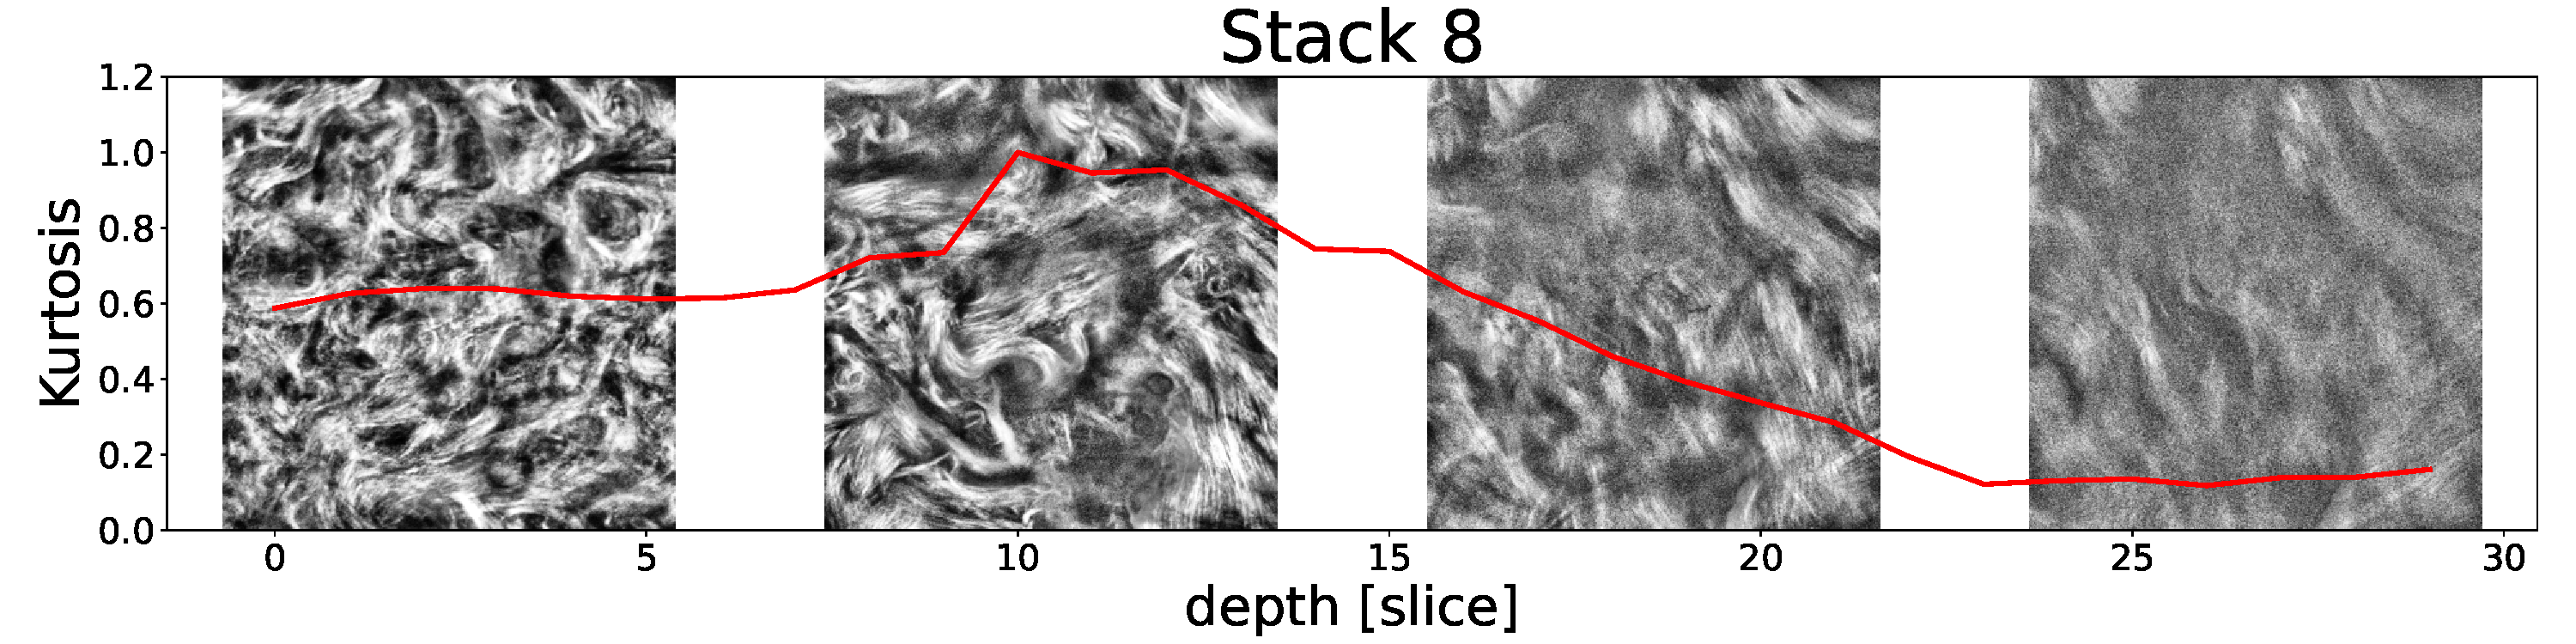
\includegraphics[width=\linewidth]{skinstression/images/kurtosis/8.pdf} \\
    % \includegraphics[width=\linewidth]{skinstression/images/kurtosis/9.pdf} \\
    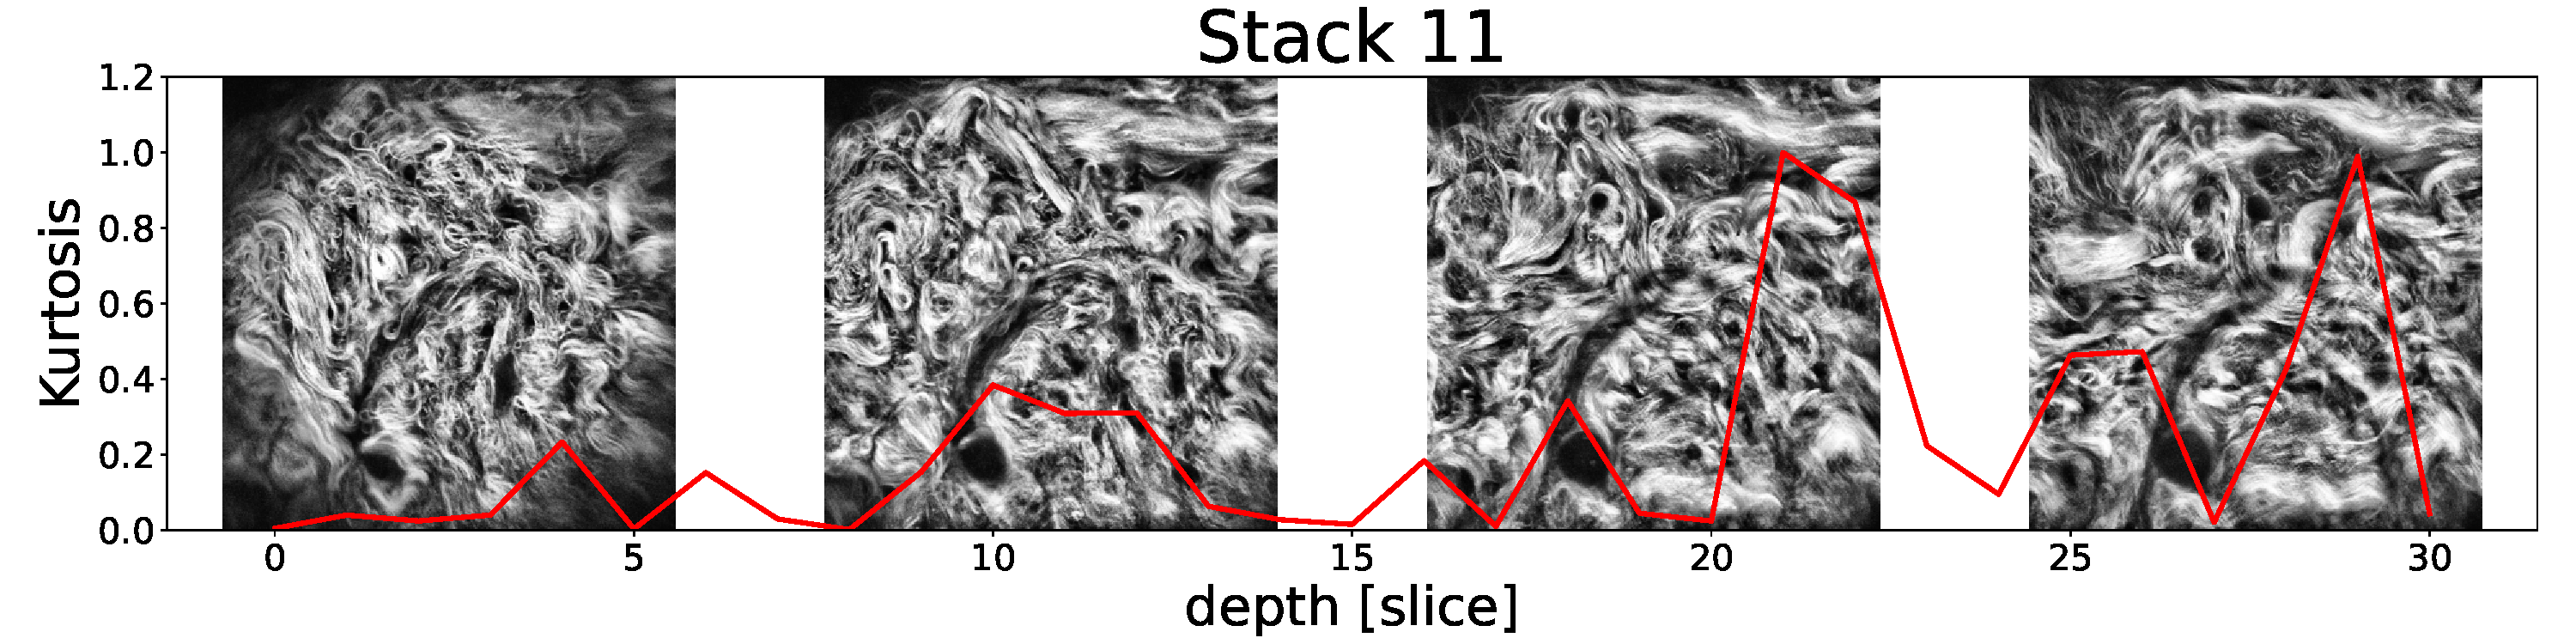
\includegraphics[width=\linewidth]{skinstression/images/kurtosis/11.pdf} \\
    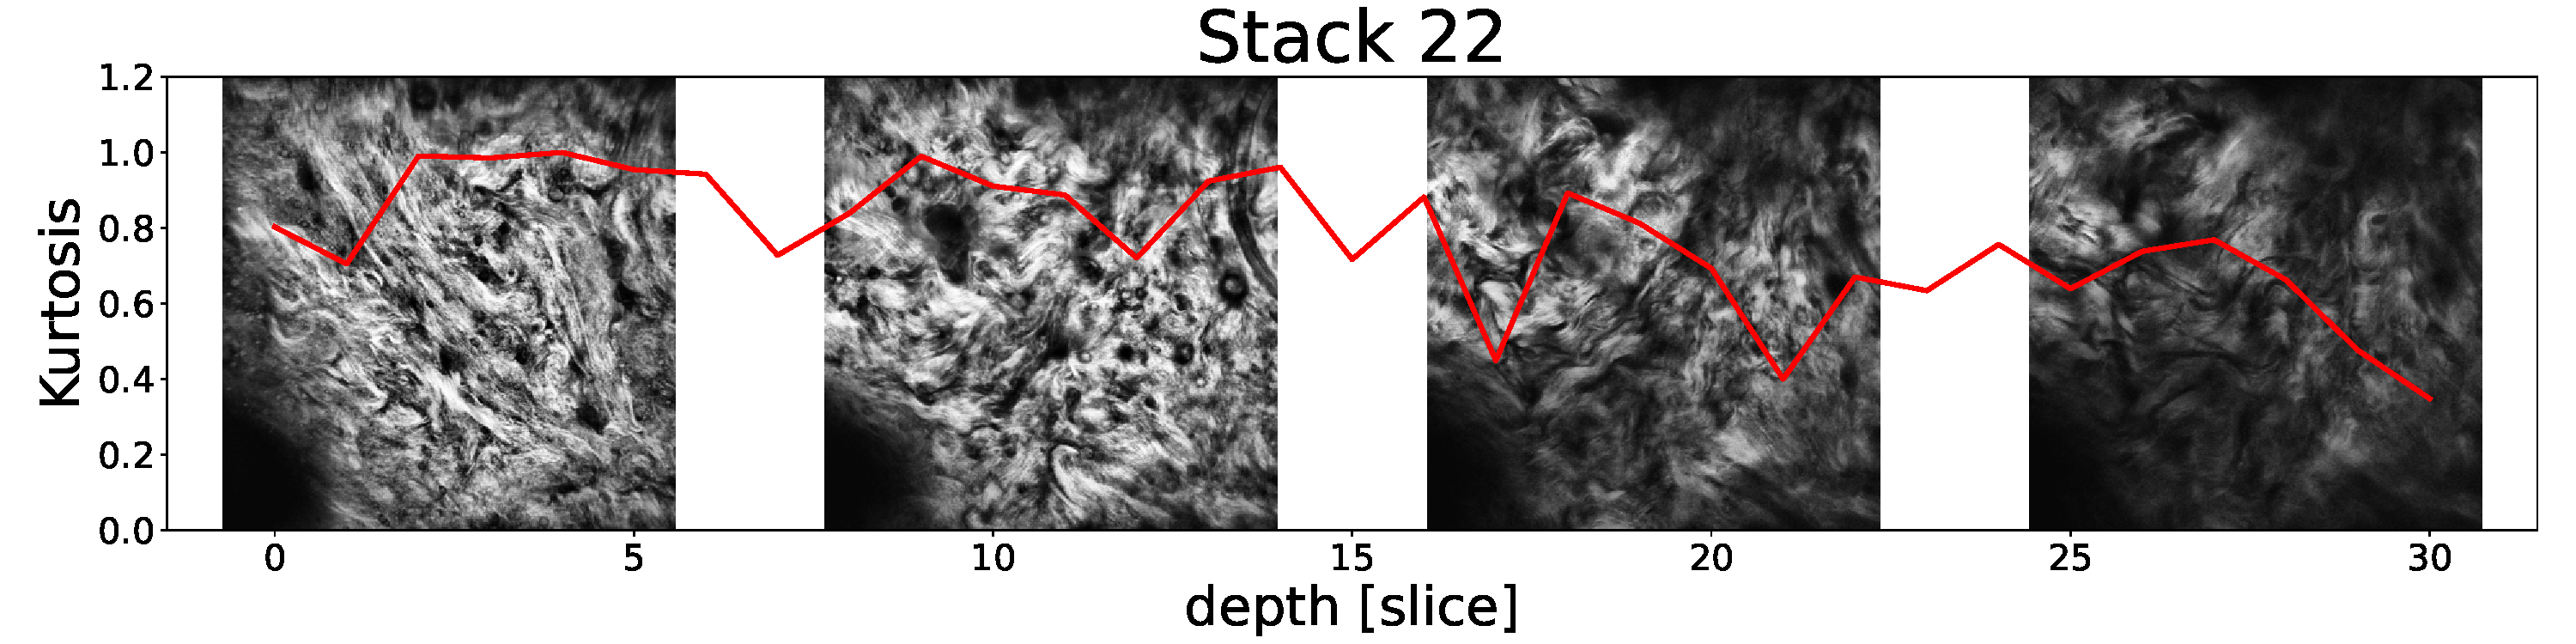
\includegraphics[width=\linewidth]{skinstression/images/kurtosis/22.pdf} \\
    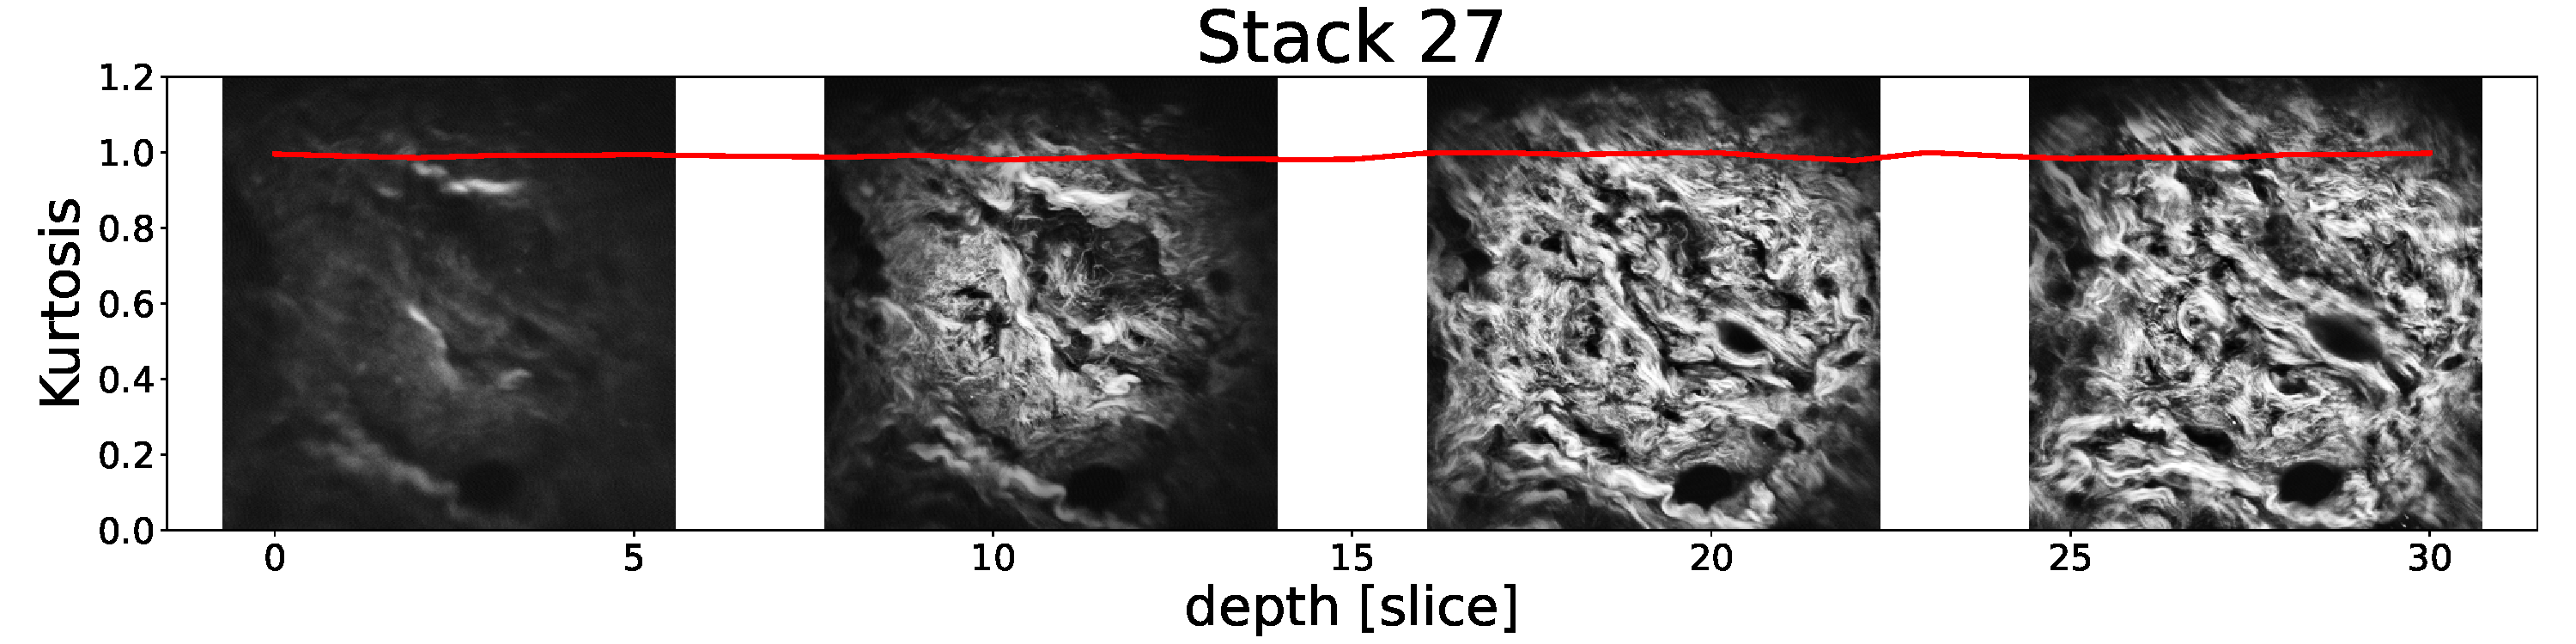
\includegraphics[width=\linewidth]{skinstression/images/kurtosis/27.pdf} \\
    % \includegraphics[width=\linewidth]{skinstression/images/kurtosis/28.pdf} \\
    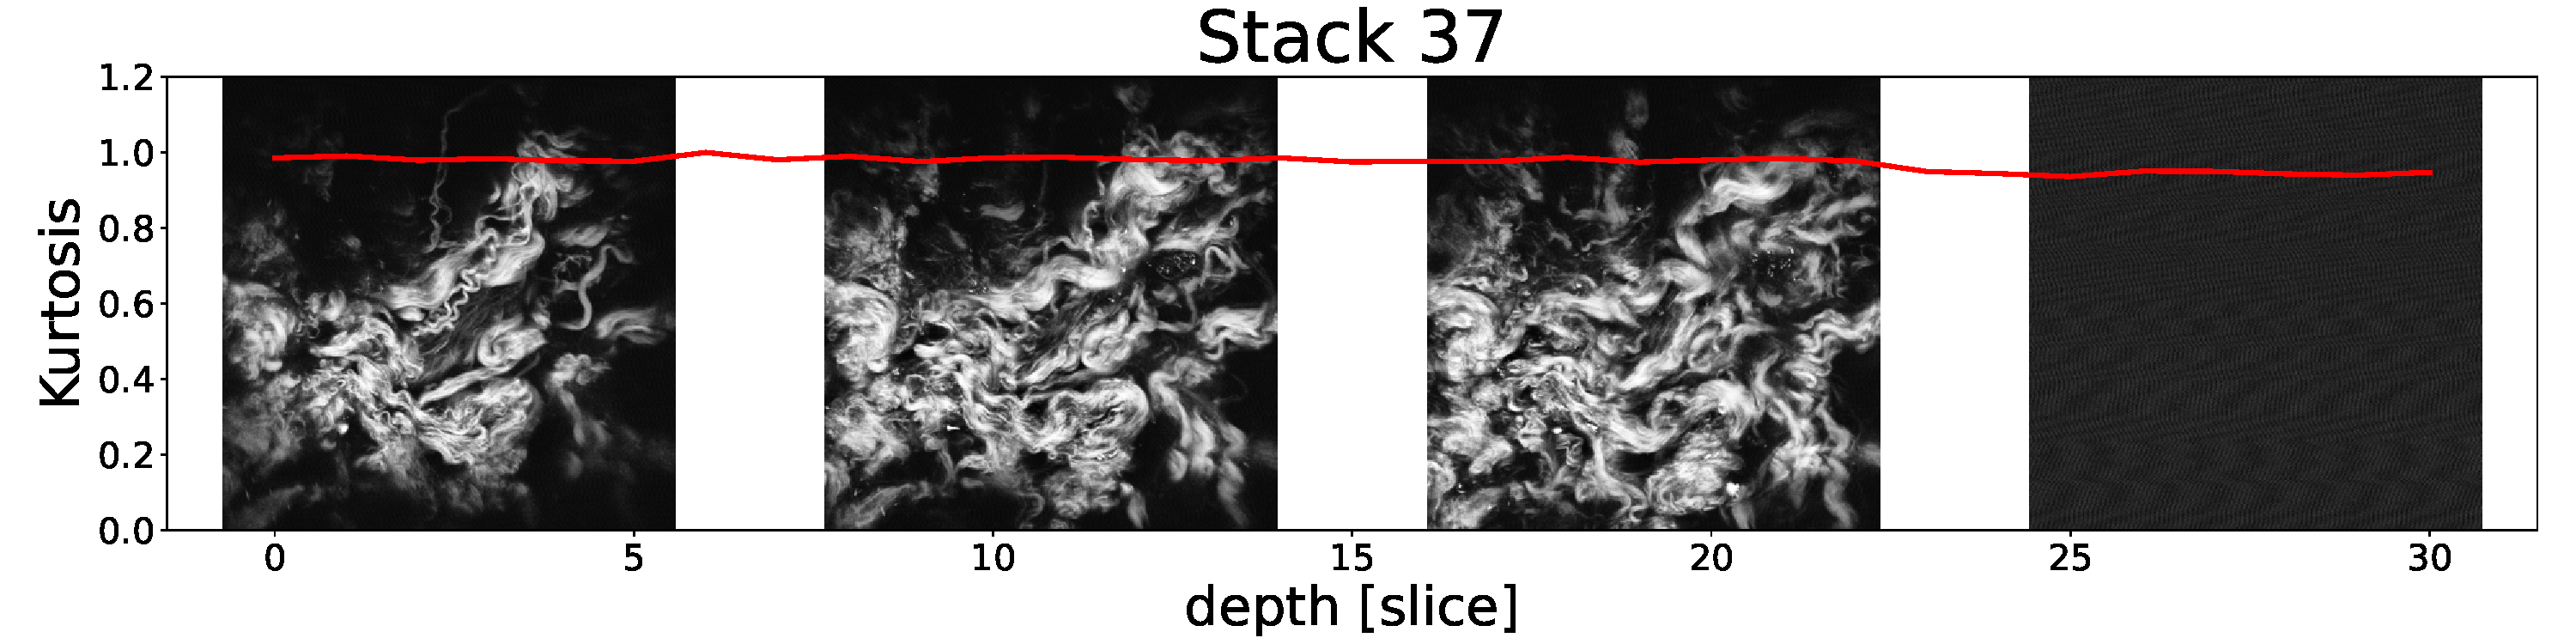
\includegraphics[width=\linewidth]{skinstression/images/kurtosis/37.pdf}
    \caption[Kurtosis vs image stack depth]{
        Kurtosis as a function of image stack depth for a representing subset.
        Four images which are equally spaced in physical units are inset.
    }
    \label{fig:skin_kurtosis_depth}
\end{figure*}

\begin{figure*}
    \centering
    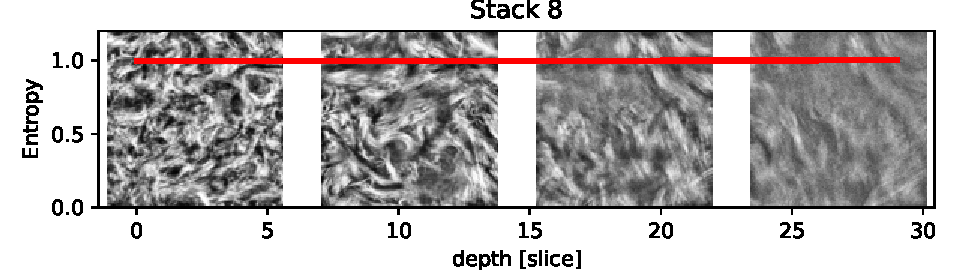
\includegraphics[width=\linewidth]{skinstression/images/entropy/8.pdf} \\
    % \includegraphics[width=\linewidth]{skinstression/images/entropy/9.pdf} \\
    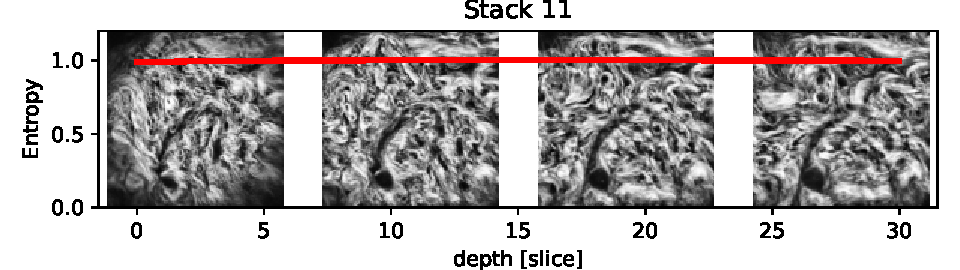
\includegraphics[width=\linewidth]{skinstression/images/entropy/11.pdf} \\
    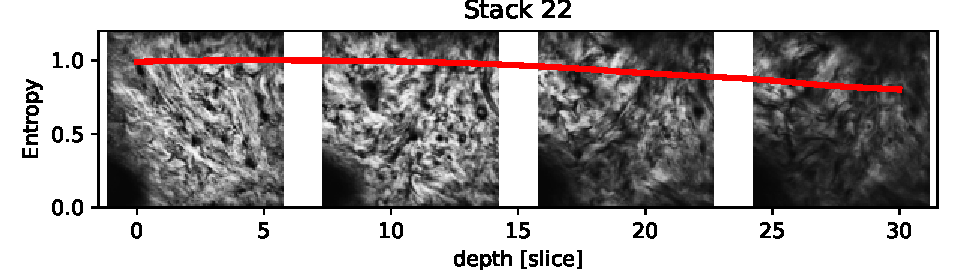
\includegraphics[width=\linewidth]{skinstression/images/entropy/22.pdf} \\
    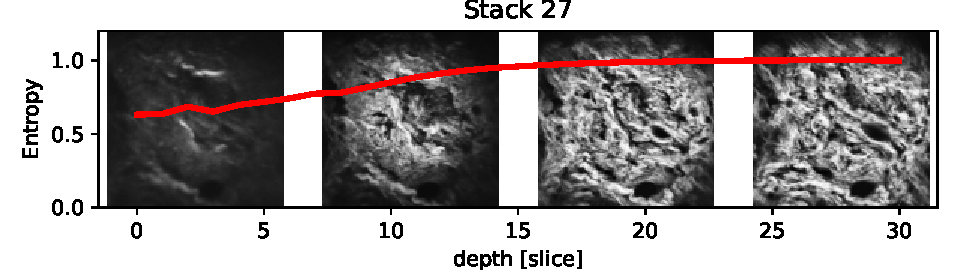
\includegraphics[width=\linewidth]{skinstression/images/entropy/27.pdf} \\
    % \includegraphics[width=\linewidth]{skinstression/images/entropy/28.pdf} \\
    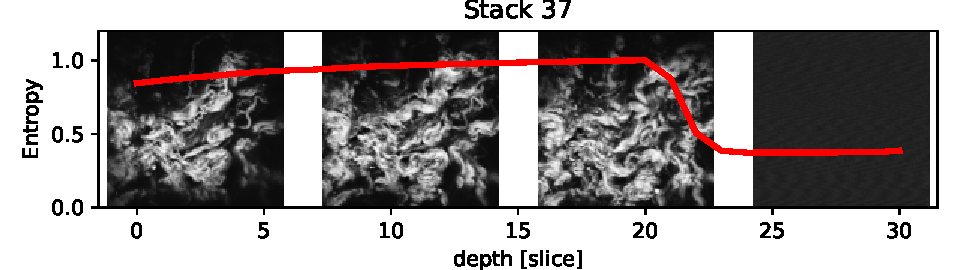
\includegraphics[width=\linewidth]{skinstression/images/entropy/37.pdf}
    \caption[Shannon entropy vs image stack depth]{
        Normalized Shannon entropy as a function of image stack depth for a representing subset.
        Four images which are equally spaced in physical units are inset.
    }
    \label{fig:skin_entropy_depth}
\end{figure*}

%%%%%%%%%%%%%%%%%%%%%%%%%%%%%%%%%%%%
% HYPERPARAMETER SEARCH
%%%%%%%%%%%%%%%%%%%%%%%%%%%%%%%%%%%%

\subsection{Hyperparameter optimization}

\subsubsection{Search 1}
The contour plot is shown in \cref{fig:skinstression-search1-contour}.
Only the loss curves of the best trial (71) is shown in \cref{fig:skinstression-search1-best-loss}.
Both training and validation loss show an increase at the learning rate restarts.

\begin{figure}
    \centering
    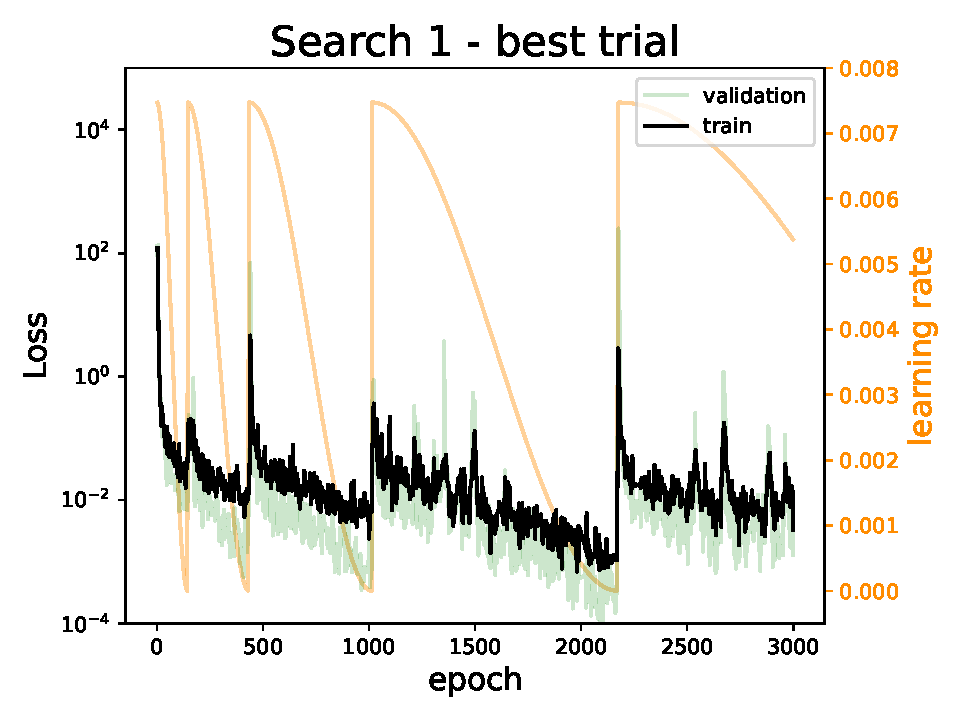
\includegraphics[]{skinstression/images/hyperparameter-search/search-1/best-trial-loss.pdf}
    \caption[Best loss curve of search 1]{
        Successive halving trial 71 of 100 has shown the best loss for search 1.
        The training loss (black) is followed by the validation loss (light green).
        The learning rate (orange) restarts explain sudden increase in loss.
    }
    \label{fig:skinstression-search1-best-loss}
\end{figure}

\begin{figure*}
    \centering
    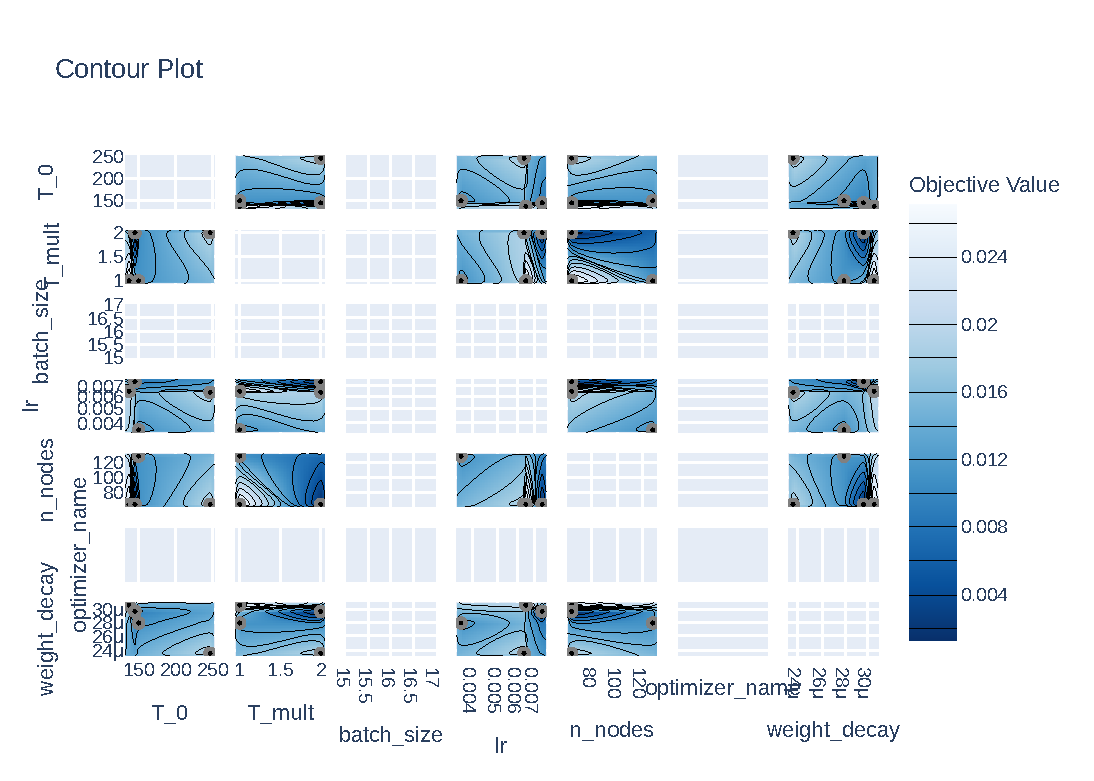
\includegraphics[angle=90,width=0.9\textheight, height=\linewidth,keepaspectratio]{skinstression/images/hyperparameter-search/search-1/contour.pdf}
    \caption[Search 1 contour plot]{
        Contour plot of search 1.
        Darker regions denote better results.
        This contour plot is only constructed from trials which have not been pruned.
    }
    \label{fig:skinstression-search1-contour}
\end{figure*}

\subsubsection{Search 2}
The contour plot is shown in \cref{fig:skinstression-search2-contour}.
Only the loss curves of the best trial (184) is shown in \cref{fig:skinstression-search2-best-loss}.
Both training and validation loss show an increase at the learning rate restarts.

\begin{figure}
    \centering
    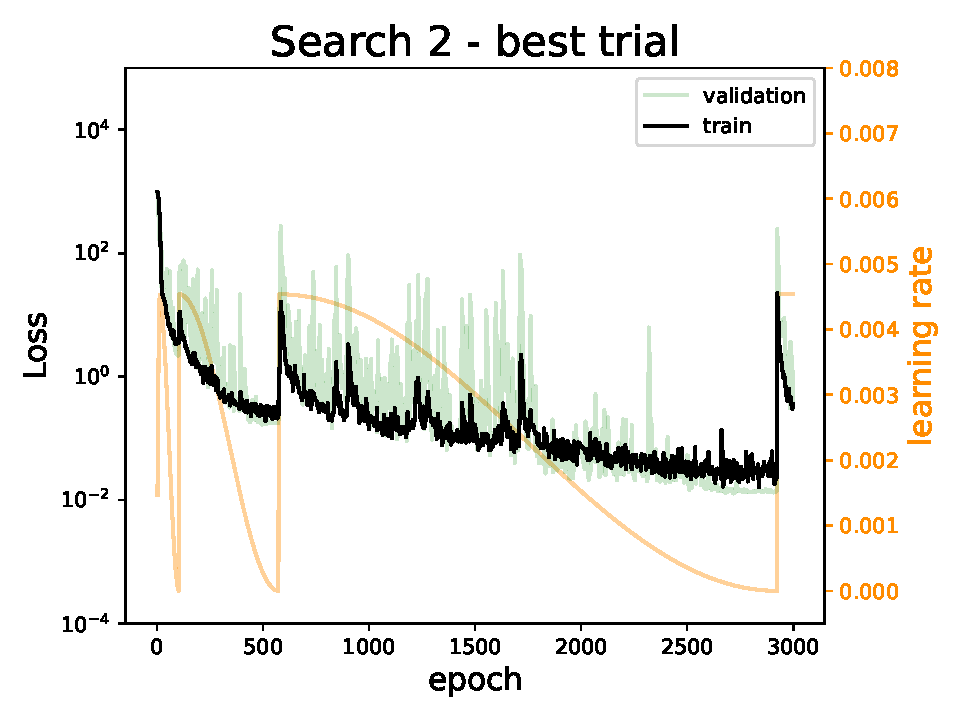
\includegraphics[]{skinstression/images/hyperparameter-search/search-2/best-trial-loss.pdf}
    \caption[Best loss curve of search 2]{
        Hyperband trial 184 of 300 has shown the best loss for search 2.
        The training loss (black) is followed by the validation loss (light green).
        The learning rate (orange) restarts explain sudden increase in loss.
    }
    \label{fig:skinstression-search2-best-loss}
\end{figure}

\begin{figure*}
    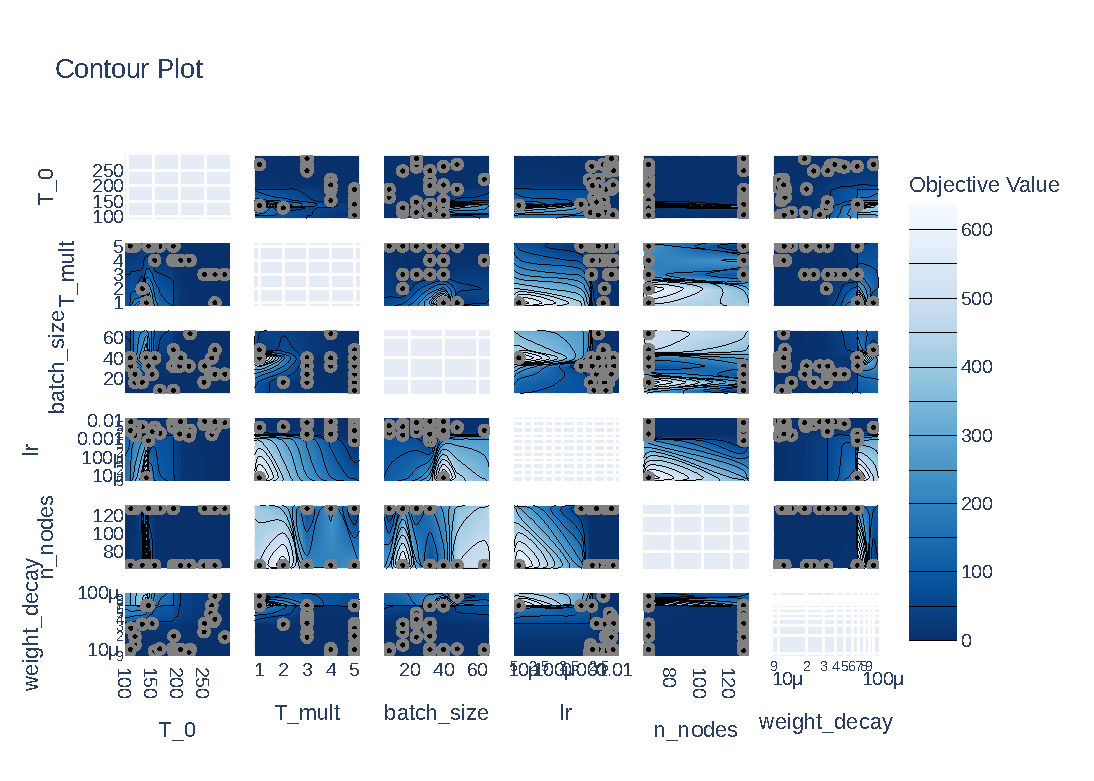
\includegraphics[angle=90,width=0.9\textheight, height=\linewidth,keepaspectratio]{skinstression/images/hyperparameter-search/search-2/contour.pdf}
    \caption[Search 2 contour plot]{
        Contour plot of search 2.
        Darker regions denote better results.
        This contour plot is only constructed from trials which have not been pruned.
    }
    \label{fig:skinstression-search2-contour}
\end{figure*}

\subsubsection{Search 3}
The contour plot is shown in \cref{fig:skinstression-search3-contour}.
Only the loss curves of the best trial (73) is shown in \cref{fig:skinstression-search3-best-loss}.
The training and validation losses diverge, showing the model overfits.

\begin{figure}
    \centering
    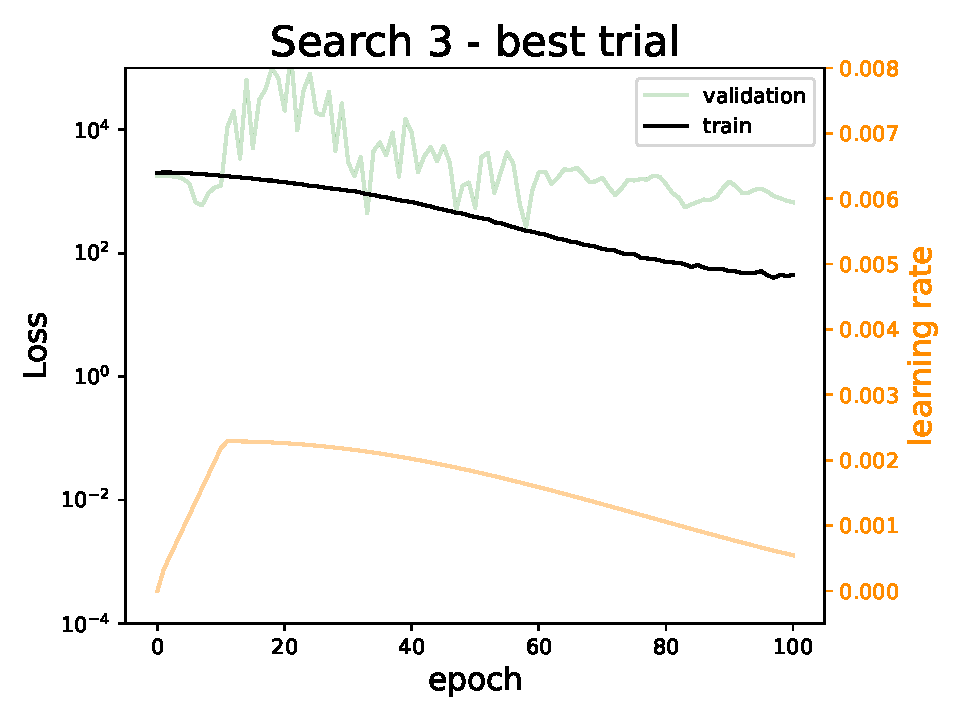
\includegraphics[]{skinstression/images/hyperparameter-search/search-3/best-trial-loss.pdf}
    \caption[Best loss curve of search 3]{
        Hyperband trial 73 of 300 has shown the best loss for search 3.
        The training loss (black) and the validation loss (light green) diverge.
        The learning rate (orange).
        The trial was pruned at epoch 100.
    }
    \label{fig:skinstression-search3-best-loss}
\end{figure}

\begin{figure*}
    \centering
    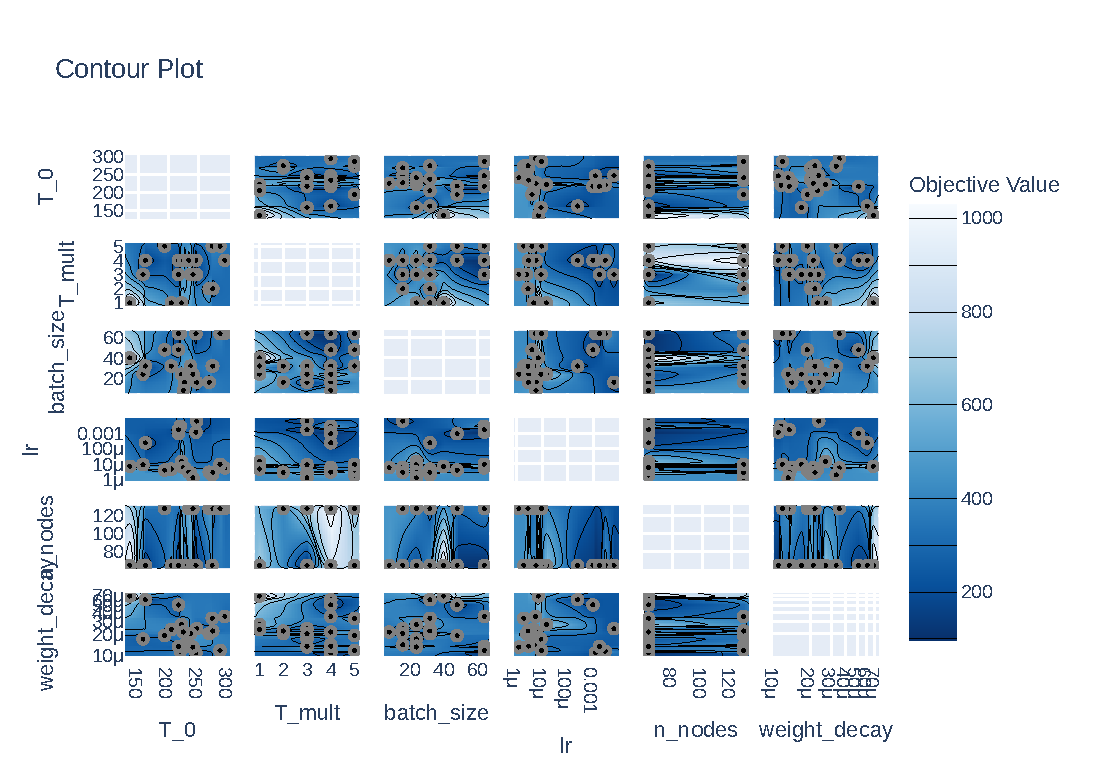
\includegraphics[angle=90,width=0.9\textheight, height=\linewidth,keepaspectratio]{skinstression/images/hyperparameter-search/search-3/contour.pdf}
    \caption[Search 3 contour plot]{
        Contour plot of search 3.
        Darker regions denote better results.
        This contour plot is only constructed from trials which have not been pruned.
    }
    \label{fig:skinstression-search3-contour}
\end{figure*}

%%%%%%%%%%%%%%%%%%
% TRAINING
%%%%%%%%%%%%%%%%%%
\subsection{Training}
Training was done on the best performing set of hyperparameters, which was found by search 1.
Search 1 yielded the lowest validation loss.
The corresponding hyperparameters in \cref{tab:conf_skin_final} were used for further training.

\begin{margintable}
    \centering
    \caption[\textsc{Skinstression} configuration]{
        \textsc{Skinstression} configuration used during training.
        Parameters are ordered by their importance, calculated with fANOVA.
        LR, WD, and BS are learning rate, weight decay and batch size, respectively.
    }
    \label{tab:conf_skin_final}
    \begin{tabular}{l c c c c c c}
        \toprule
        Param.               & Value         & Imp. \\
        \midrule
        {LR}                 & 0.00747       & 0.41 \\
        {$T_0$}              & 145           & 0.24 \\
        {WD}                 & \num{2.97e-5} & 0.22 \\
        {$n_\mathrm{nodes}$} & 64            & 0.08 \\
        {$T_\mathrm{mult}$}  & 2             & 0.05 \\
        {BS}                 & 16            & 0.00 \\
        \bottomrule
    \end{tabular}
\end{margintable}

Three trainings were performed.
For every training, the 10, 20, and 30 images with highest entropy were selected to exclude any noisy images.
The loss curves are shown in \cref{fig:skinstression-training}.
The lowest validation losses are shown in \cref{tab:skin_train_102030}.
Overall, the model trained with 20 images shows the lowest total loss.
This model will be used during testing.

To verify performance of training, the stress-strain curves of a random training batch are plotted with the raw data in \cref{fig:skinstression-train-logistic-curves}.


\begin{figure}
    \centering
    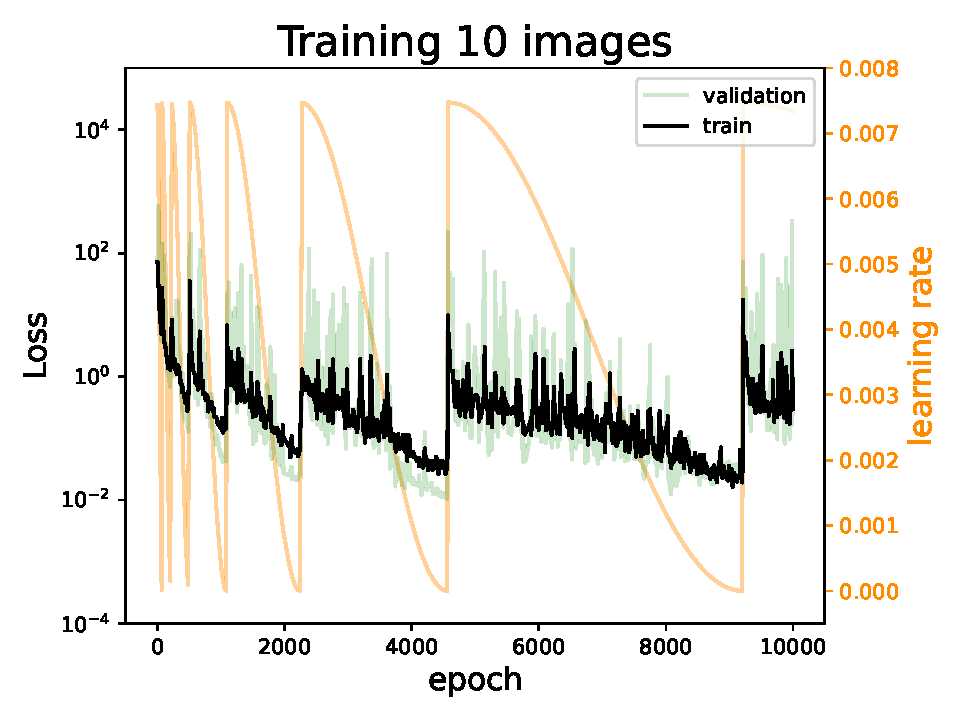
\includegraphics[]{skinstression/images/training/Training_10_images.pdf} \\
    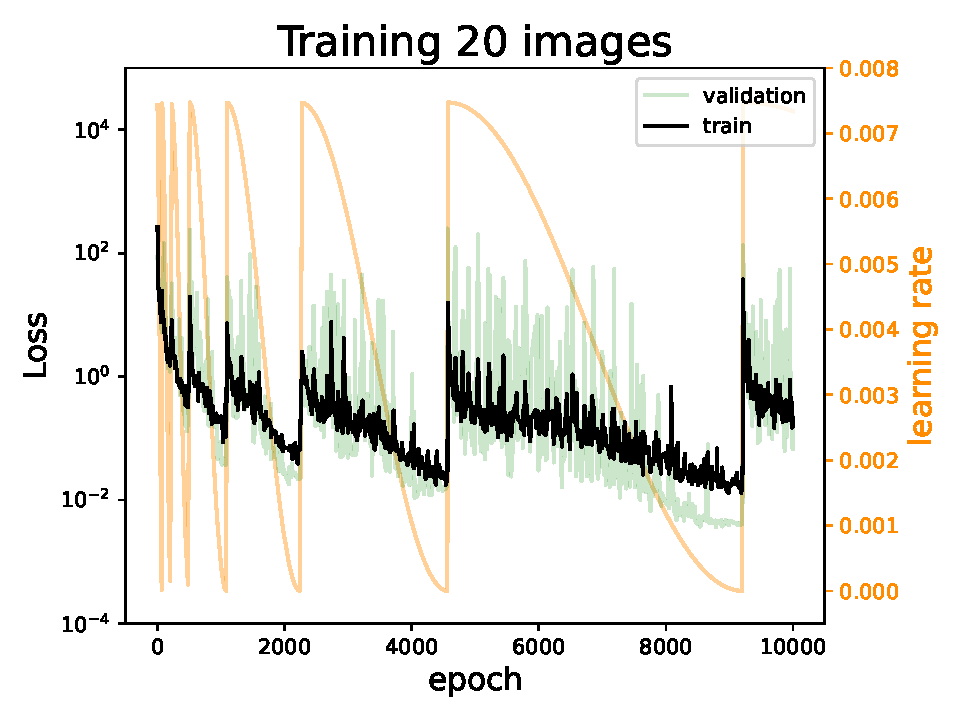
\includegraphics[]{skinstression/images/training/Training_20_images.pdf} \\
    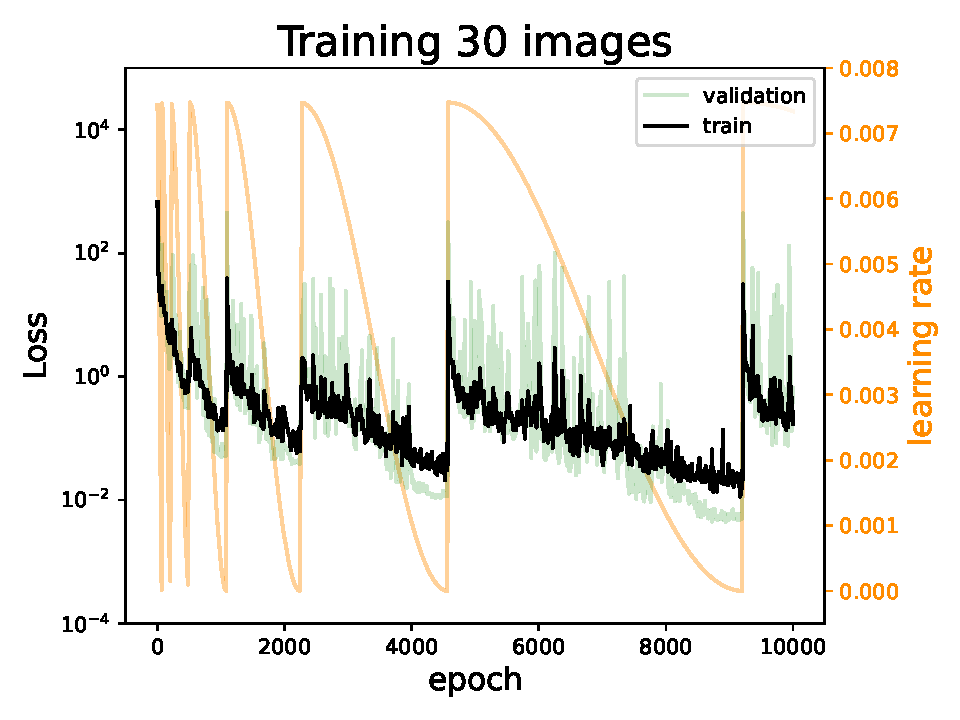
\includegraphics[]{skinstression/images/training/Training_30_images.pdf}
    \caption[Training with 10 images]{
        Training using 10, 20, and 30 images respectively.
        The training loss (black) is followed by the validation loss (light green).
        The learning rate (orange) restarts explain sudden increase in loss.
    }
    \label{fig:skinstression-training}
\end{figure}

\begin{margintable}
    \centering
    \caption[Lowest validation loss per $N_\mathrm{best}$ images]{
        Lowest validation loss per $N_\mathrm{best}$ images.
        The training using 20 images has the lowest validation loss.
    }
    \label{tab:skin_train_102030}
    \begin{tabular}{c c}
        \toprule
        \# Images   & Validation loss \\
        \midrule
        10          & 0.0097          \\
        \textbf{20} & \textbf{0.0035} \\
        30          & 0.0040          \\
        \bottomrule
    \end{tabular}
\end{margintable}

\begin{figure*}
    \centering
    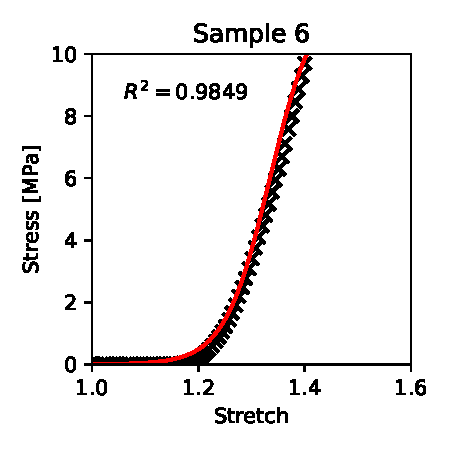
\includegraphics[width=0.24\linewidth]{skinstression/images/training/sample_6_0.pdf}
    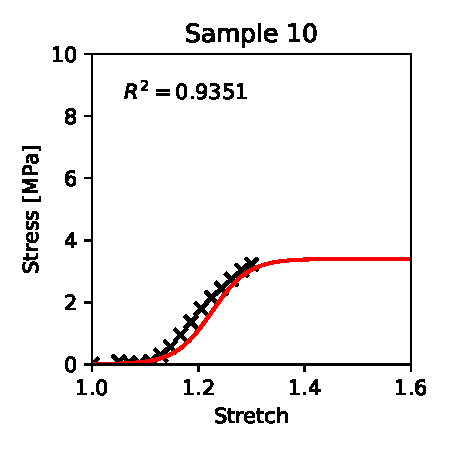
\includegraphics[width=0.24\linewidth]{skinstression/images/training/sample_10_0.pdf}
    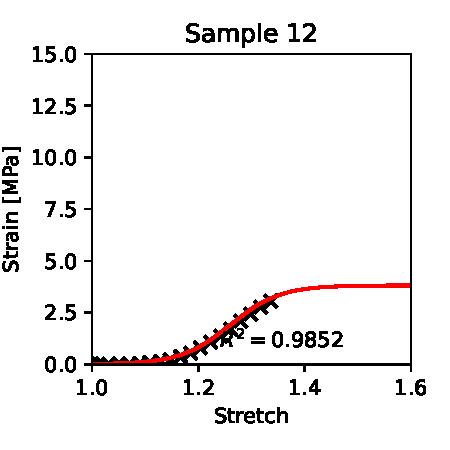
\includegraphics[width=0.24\linewidth]{skinstression/images/training/sample_12_0.pdf}
    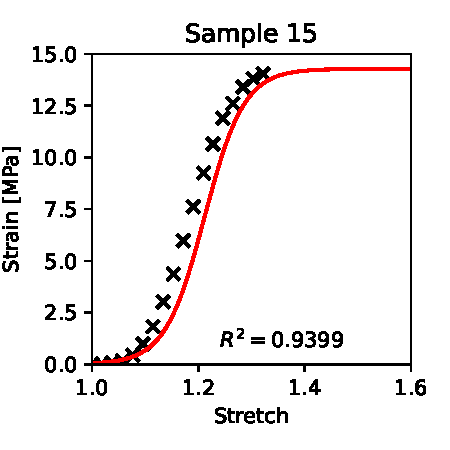
\includegraphics[width=0.24\linewidth]{skinstression/images/training/sample_15_0.pdf} \\
    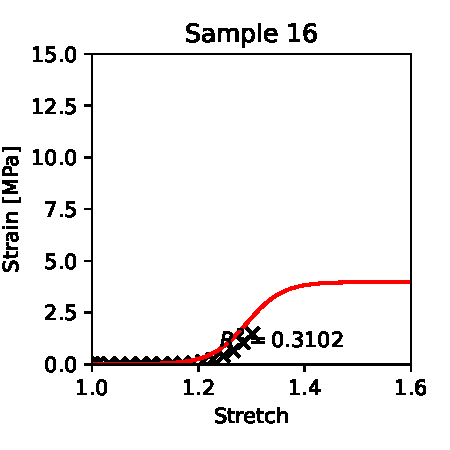
\includegraphics[width=0.24\linewidth]{skinstression/images/training/sample_16_0.pdf}
    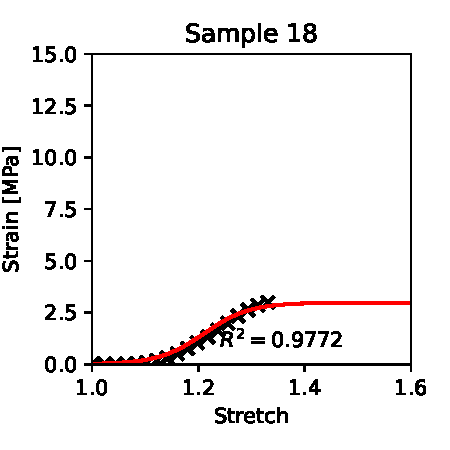
\includegraphics[width=0.24\linewidth]{skinstression/images/training/sample_18_0.pdf}
    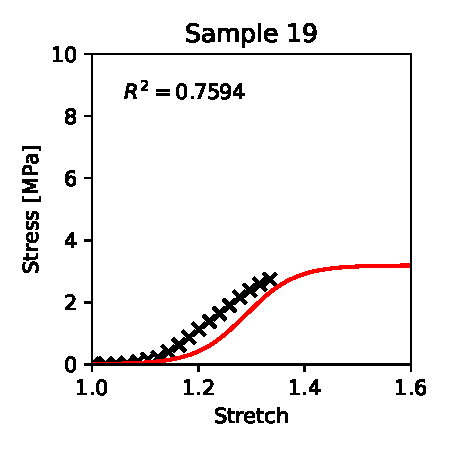
\includegraphics[width=0.24\linewidth]{skinstression/images/training/sample_19_0.pdf}
    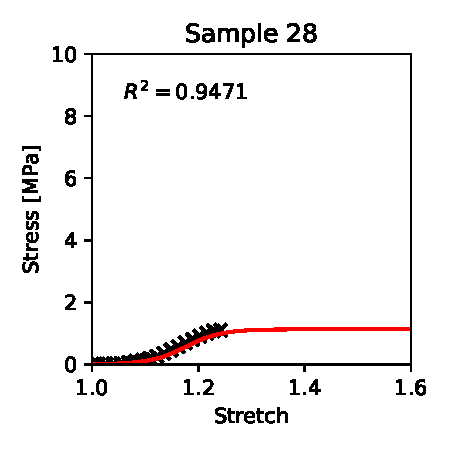
\includegraphics[width=0.24\linewidth]{skinstression/images/training/sample_28_0.pdf} \\
    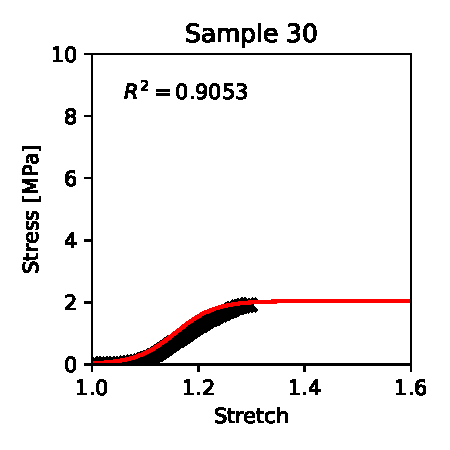
\includegraphics[width=0.24\linewidth]{skinstression/images/training/sample_30_0.pdf}
    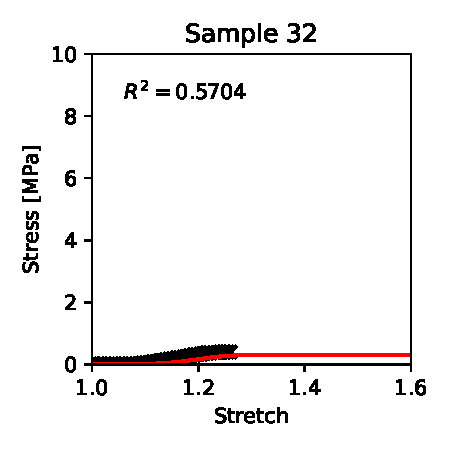
\includegraphics[width=0.24\linewidth]{skinstression/images/training/sample_32_0.pdf}
    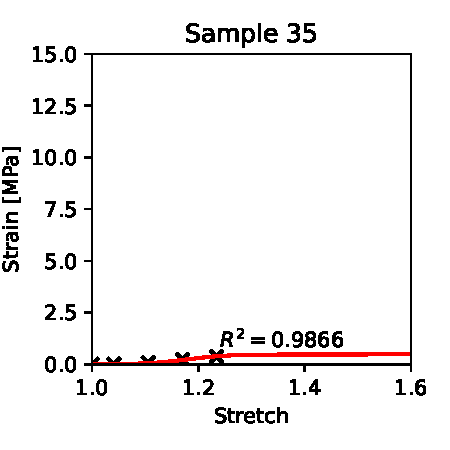
\includegraphics[width=0.24\linewidth]{skinstression/images/training/sample_35_0.pdf}
    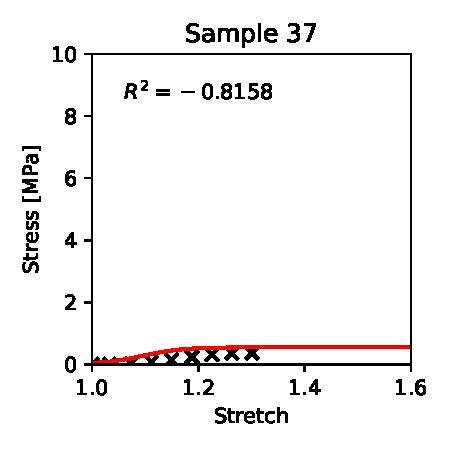
\includegraphics[width=0.24\linewidth]{skinstression/images/training/sample_37_0.pdf} \\
    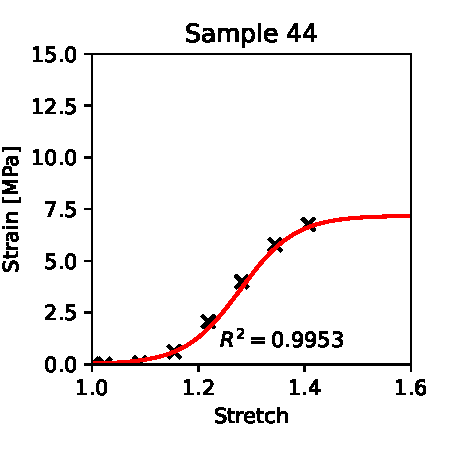
\includegraphics[width=0.24\linewidth]{skinstression/images/training/sample_44_1.pdf}
    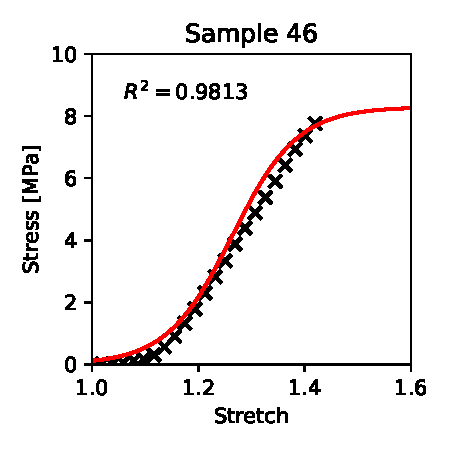
\includegraphics[width=0.24\linewidth]{skinstression/images/training/sample_46_0.pdf}
    \caption[Training results]{
        Results of a random training batch.
        Raw mechanical measurement without error bars ($\times$) are shown together with the AI fit (red).
        Performance is quantified by $R^2$.
    }
    \label{fig:skinstression-train-logistic-curves}
\end{figure*}

\subsection{Testing}
The results of the best performing images in the test set are shown in \cref{fig:skinstression-test}.
The higher $R^2$, the better the performance.

\begin{figure*}
    \centering
    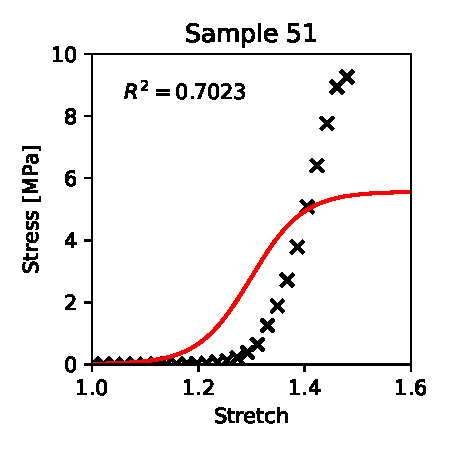
\includegraphics[width=0.24\linewidth]{skinstression/images/testing/sample_51_11.pdf}
    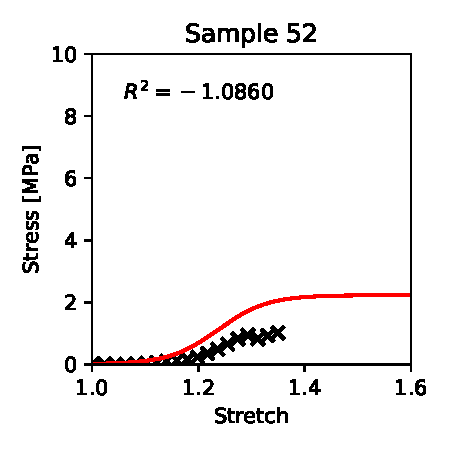
\includegraphics[width=0.24\linewidth]{skinstression/images/testing/sample_52_15.pdf}
    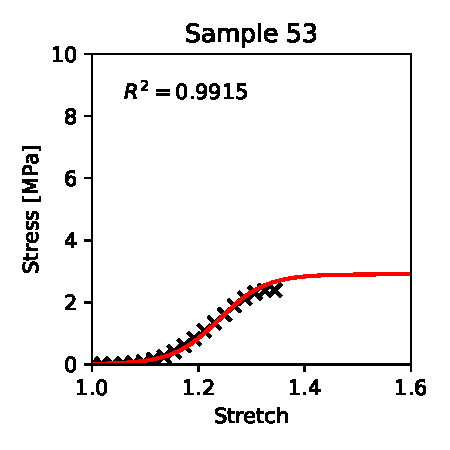
\includegraphics[width=0.24\linewidth]{skinstression/images/testing/sample_53_12.pdf}
    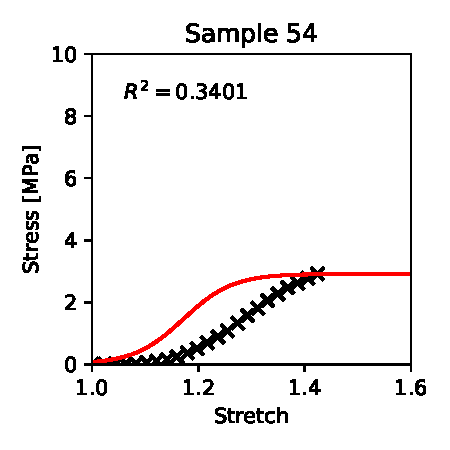
\includegraphics[width=0.24\linewidth]{skinstression/images/testing/sample_54_17.pdf} \\
    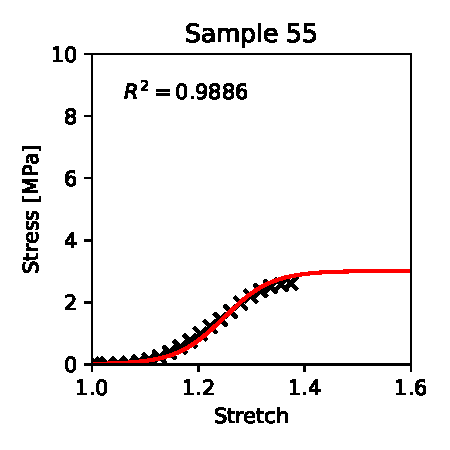
\includegraphics[width=0.24\linewidth]{skinstression/images/testing/sample_55_10.pdf}
    \includegraphics[width=0.24\linewidth]{skinstression/images/testing/sample_56_9.pdf}
    \includegraphics[width=0.24\linewidth]{skinstression/images/testing/sample_57_19.pdf}
    \includegraphics[width=0.24\linewidth]{skinstression/images/testing/sample_58_17.pdf} \\
    \includegraphics[width=0.24\linewidth]{skinstression/images/testing/sample_59_16.pdf}
    \includegraphics[width=0.24\linewidth]{skinstression/images/testing/sample_60_10.pdf}
    \includegraphics[width=0.24\linewidth]{skinstression/images/testing/sample_61_18.pdf}
    \caption[Test results]{
        Results of the best performing image per sample are shown.
        Performance is quantified by $R^2$.
    }
    \label{fig:skinstression-test}
\end{figure*}

\subsection{Model specification}
The foundational neural network is described in \cref{fig:model}.
x neural networks combined make up the final model.
The output of the model is the average of the outputs of the individual models.
It accepts a batch of images as input and outputs a vector $(i, \sigma_\mathrm{max}, E_\mathrm{max}, \gamma_c)$,
where $i$ denotes the $i$th image of the batch.


\subsection{Usability}
The prediction AI may be used for three purposes.
One purpose is to skip the mechanical measurement on skin tissue and immediately get an estimation of stretch properties.
Another is to match stretch information to physical features present in the collagen fiber networks.
The model should not be used as validation for the mechanical measurement, as it is trained and tested on a dataset with small variance.

Input data should be assessed on quality.
A measure of quality is Shannon entropy, which is used in this study.
However, the model may benefit from other quality measures.
The user should experiment what measure works best.
The application does allow to only select the top $N_\mathrm{best}$ images.

The model only accepts batches of two-dimensional $500x500\,\unit{px}$ images.
The user should separate any higher-dimensional data and crop the images to fit the model.

\subsubsection{Explainability}

\subsubsection{Occlusion}
Algorithmically occluded images have been presented to the model to obtain attributions at the pixel level.
For a summary of the test set, they are shown in blended heatmaps in \cref{fig:skin_occlusion}.
\cref{fig:skin_occlusion_53} shows attribution maps for all test images of sample 53.

% \begin{figure*}
%     \ContinuedFloat
%     \centering
%     \includegraphics[width=\linewidth]{skinstression/images/explainability/occlusion/0.pdf} \\
%     \raggedleft Continued on next page.
% \end{figure*}
\begin{figure*}
    % \ContinuedFloat
    \centering
    \includegraphics[width=\linewidth]{skinstression/images/explainability/occlusion/summary_test_0.pdf}
    \caption[Original image and attribution heat maps]{
        Original image and attribution heat maps.
        Attributions are blended with the original image.
        Attributions were calculated using $20\times 20\unit{px}$ occlusion.
        Color scale is from \numrange{-3}{3} units, and is linear from \qtyrange{-0.1}{0.1}{\mega\pascal}, \qtyrange{-0.1}{0.1}{\mega\pascal\per\stretch}, and \qtyrange{-0.001}{0.001}{\stretch}.
        Mean $\pm$ standard deviation are inset.
        Zoom in in the digital version for details.
    }
    \label{fig:skin_occlusion}
\end{figure*}


\begin{figure*}
    \ContinuedFloat
    \centering
    \includegraphics[width=\linewidth]{skinstression/images/explainability/occlusion/summary_53_0.pdf} \\
    \raggedleft Continued on next page.
\end{figure*}
\begin{figure*}
    % \ContinuedFloat
    \centering
    \includegraphics[width=\linewidth]{skinstression/images/explainability/occlusion/summary_53_1.pdf}
    \caption[Original image and attribution heat maps for sample 53]{
        Original image and attribution heat maps for sample 53.
        Attributions are blended with the original image.
        Attributions were calculated using $20\times 20\unit{px}$ occlusion.
        Green and red show which parts attribute to under- and overestimations, compared to output calculated from an unoccluded image.
        Color scale is from \numrange{-1.5}{1.5} units, and is linear from \qtyrange{-0.1}{0.1}{\mega\pascal}, \qtyrange{-0.1}{0.1}{\mega\pascal\per\stretch}, and \qtyrange{-0.001}{0.001}{\stretch}.
        Mean $\pm$ standard deviation are inset.
        Zoom in in the digital version for details.
    }
    \label{fig:skin_occlusion_53}
\end{figure*}

\subsubsection{Adversarial attack}
\Cref{fig:attack_occlusion} shows attribution maps for all outputs to compare attacked images with the original image.
\Cref{fig:pred_output_attack} shows the predicted logistic curves for the attacked images and the original image.

\begin{figure*}
    \centering
    \includegraphics[width=\linewidth]{skinstression/images/attack/attack-viz.pdf} \\
    \includegraphics[width=\linewidth]{skinstression/images/attack/holes-occlusion-0.pdf} \\
    \includegraphics[width=\linewidth]{skinstression/images/attack/holes-occlusion-1.pdf} \\
    \includegraphics[width=\linewidth]{skinstression/images/attack/holes-occlusion-2.pdf}
    \caption[Occlusion on attacked image]{
        Top row shows a visualization of the two attacks.
        The middle image has holes filled with white.
        The right image has duplicates of one hole.
        The next rows show occlusion attribution maps for all outputs.
        Color scales are equal to \cref{fig:skin_occlusion_53}.
    }
    \label{fig:attack_occlusion}
\end{figure*}

\begin{figure}
    \centering
    \includegraphics{skinstression/images/attack/holes.pdf}
    \caption[Prediction output after hole attack]{
        Prediction output after hole attack.
    }
    \label{fig:pred_output_attack}
\end{figure}